\documentclass[12pt,a4paper]{report}
\usepackage[utf8]{inputenc}
\usepackage[T1]{fontenc}
\usepackage{lmodern}
\usepackage{caption}
\captionsetup{font=footnotesize}
\usepackage{amsmath}
%\usepackage{algorithm}
\usepackage{listings}
%\usepackage{standalone}
%\usepackage{algpseudocode}
\usepackage[linesnumbered,lined,boxed,commentsnumbered]{algorithm2e}
\SetKw{KwBy}{by} 
\newcommand\mycommfont[1]{\footnotesize\ttfamily{#1}}
\SetCommentSty{mycommfont}
\usepackage{verbatim}
\usepackage{tabularx}
%\usepackage{program}
%\input{externaldoc}
%\input{verticalblock}
%\algrenewcommand\algorithmicindent{1.0em}
\usepackage{minitoc}
\usepackage{float}
\usepackage{hyperref}
\usepackage{physics}
\usepackage{color}
\usepackage{subfiles}
\usepackage{pdfpages}
\usepackage{centernot}
\usepackage[ED=SDM-PMat, Ets=UT3]{tlsflyleaf}

\hypersetup{
 colorlinks=true,
 linkcolor=blue,
 filecolor=blue,
 urlcolor=blue,
 citecolor=blue
}
\usepackage{mathpazo,libertine}



\newcommand{\alert}[1]{\textcolor{red}{#1}}
\newcommand{\Hij}[3][\hat{H}]{\mel{#2}{#1}{#3}}
%\newcommand{\ket}[1]{| #1 \rangle}

%sizes
\newcommand{\Ndet}{{N_\text{det}}}
\newcommand{\Ngen}{{N_\text{gen}}}
\newcommand{\Nsel}{{N_\text{sel}}}
\newcommand{\Norb}{{N_\text{orb}}}
\newcommand{\Nelec}{{N_\text{elec}}}
\newcommand{\Nalpha}{{N_\text{elec}^\alpha}}
\newcommand{\Nbeta}{{N_\text{elec}^\beta}}
\newcommand{\Nint}{{N_\text{int}}}
\newcommand{\Nst}{{N_\text{states}}}
\newcommand{\Ndav}{{N_\text{dav}}}
\newcommand{\Nperm}{{N_\text{perm}}}
\newcommand{\Na}{{N_\alpha}}
\newcommand{\Nb}{{N_\beta}}
\newcommand{\Ne}{{N_\text{elec}}}
\newcommand{\NFCI}{N_\text{FCI}}

%bitmasks
\newcommand{\bit}[1]{{\texttt{#1}}}
\newcommand{\bitI}{{\texttt{I}}}
\newcommand{\bitP}{{\texttt{P}}}
\newcommand{\bitJ}{{\bit{J}}}
\newcommand{\bitK}{{\bit{K}}}
\newcommand{\bitx}[2]{{\texttt{#1}_{#2}}}
\newcommand{\bitIsigma}{{\bitx{I}{\sigma}}}
\newcommand{\bitPsigma}{{\bitx{P}{\sigma}}}
\newcommand{\binary}[1]{{#1_{\mathtt{2}}}}
\newcommand{\TRUE}{{\text{\texttt{TRUE}}}}
\newcommand{\FALSE}{{\text{\texttt{FALSE}}}}


%acronyms
\newcommand{\HF}{{\text{HF}}}
\newcommand{\QP}{{ \textsc{Quantum Package} }}

%energies
\newcommand{\EDMC}{E_\text{DMC}}
\newcommand{\EPT}{E_\text{PT2}}
\newcommand{\Ecor}{E_\text{corr}}
\newcommand{\Evar}{E_\text{var}}
\newcommand{\EFCI}{E_\text{FCI}}
\newcommand{\ECI}{E_\text{CI}}
\newcommand{\E}[1]{E_{#1}}


%operators
\newcommand{\vac}{ {\ket{}} }
\newcommand{\ac}[1]{a^\dagger_{#1}}
\newcommand{\an}[1]{a_{#1}}
\newcommand{\hH}{\Hat{H}}
\newcommand{\ordering}{{\hat{\mathcal{O}}}}
\newcommand{\phase}[2]{{\Phi \qty(#1 \rightarrow #2)}}

%determinants
\newcommand{\kalpha}{{\ket{\alpha}}}
\newcommand{\kbeta}{{\ket{\beta}}}
\newcommand{\ki}{{\ket{i}}}
\newcommand{\kj}{{\ket{j}}}
\newcommand{\kI}{{\ket{I}}}
\newcommand{\kIp}{{\ket{I'}}}
\newcommand{\kJ}{{\ket{J}}}
\newcommand{\kJp}{{\ket{J'}}}
\newcommand{\kK}{{\ket{J}}}
\newcommand{\occ}[2]{{\text{occ}(#1,#2)}}

%excitation
\newcommand{\excdet}[2]{{\hat{T}_{#1 \rightarrow #2}}}
\newcommand{\excorb}[2]{{\hat{T}_{#1}^{#2}}}

%space
\newcommand{\br}{{\mathbf{r}}}
\newcommand{\bR}{{\mathbf{R}}}

%Fortran
\newcommand{\POPCNT}[1]{\text{\texttt{POPCNT}}(#1)}
\newcommand{\TRAILZ}[1]{\text{\texttt{TRAILZ}}(#1)}
\newcommand{\IBSET}[1]{\text{\texttt{IBSET}}(#1)}
\newcommand{\IBCLR}[2]{\text{\texttt{IBCLR}}(#1,#2)}
\newcommand{\BTEST}[2]{\text{\texttt{BTEST}}(#1,#2)}
\newcommand{\ISHFT}[2]{\text{\texttt{ISHFT}}(#1,#2)}
\newcommand{\IAND}[2]{\text{\texttt{IAND}}(#1,#2)}
\newcommand{\IEOR}[2]{\text{\texttt{IEOR}}(#1,#2)}
\newcommand{\IOR}[2]{\text{\texttt{IOR}}(#1,#2)}
\newcommand{\NOT}[1]{\text{\texttt{NOT}}(#1)}

\newcommand{\popcnt}[1]{\norm{#1}}
\newcommand{\trailz}[1]{\text{trailing\_zeros}(#1)}
\newcommand{\ibset}[1]{\text{bit\_set}(#1)}
\newcommand{\ibclr}[2]{\text{bit\_clear}(#1,#2)}
\newcommand{\btest}[2]{\text{bit\_test}(#1,#2)}
\newcommand{\ishft}[2]{\text{shift\_left}(#1,#2)}
\newcommand{\iand}[2]{#1 \wedge #2}
\newcommand{\ieor}[2]{#1 \oplus #2}
\newcommand{\ior}[2]{#1 \vee #2}
%\newcommand{\not}[1]{{\neg #1}}

%Sets
\newcommand{\set}[1]{{\mathcal{#1}}}
\newcommand{\setx}[2]{{\mathcal{#1}_{#2}}}
\newcommand{\setI}{\set{I}}
\newcommand{\setJ}{\set{J}}

%matrices and vectors
\newcommand{\mH}{\mathbf{H}}
\newcommand{\mc}{\mathbf{c}}



%centering in tables
\newcommand{\tabc}[1]{\multicolumn{1}{c}{#1}}




%%%%%
% À mettre dans le préambule (avant \begin{document})
%%%%%
%% Titre, auteur, date, laboratoire, cotutelle
%\title{Development and parallel implementation of Selected Configuration Interaction methods}
\title{Développement et implémentation parallèle de méthodes d'interaction de configurations sélectionnées}
\author{Yann GARNIRON}
\defencedate{15/11/2018}
\lab{Laboratoire de Chimie et Physique Quantiques (UMR 5626)}
%\cotutelle{Institut de cotutelle}

%% Directeur(s) de thèse
\nboss{1}                                    % Nombre de directeur(s) de thèse
\makesomeone{boss}{1}{Anthony SCEMAMA}{Ingénieur de Recherche}{Directeur} % Sera affiché en premier
%% Referee
\nreferee{2}
\makesomeone{referee}{1}{Philippe CARBONNIERE}{Professeur d'Université}{Rapporteur}
\makesomeone{referee}{2}{Jean-Philip PIQUEMAL}{Professeur d'Université}{Rapporteur}
%% Jury
\njudge{2}
\makesomeone{judge}{1}{Nathalie GUIHERY}{Professeure d'Université}{Président du Jury}
\makesomeone{judge}{2}{Nicolas RENON}{Ingénieur de Recherche}{Examinateur}
%\makesomeone{judge}{3}{Troisième MEMBRE}{Chargé de Recherche}{}


\usepackage[square,sort,comma,numbers]{natbib}
\usepackage{graphicx}


\lstset{% setup listings
        language=Fortran,% set programming language
        basicstyle=\ttfamily\footnotesize,% basic font style
%       keywordstyle=\bfseries,% keyword style
%        commentstyle=\ttfamily\itshape,% comment style
%       numbers=left,% display line numbers on the left side
%       numberstyle=\scriptsize,% use small line numbers
%       numbersep=10pt,% space between line numbers and code
        tabsize=2,% sizes of tabs
        showstringspaces=false,% do not replace spaces in strings by a certain character
        captionpos=b,% positioning of the caption below
        breaklines=true,% automatic line breaking
        escapeinside={(*}{*)},% escaping to LaTeX
        extendedchars=false,% prohibit extended chars (chars of codes 128--255)
        otherkeywords={assert,
            POPCNT, ISHFT, IBCLR, IOR, IEOR, TRAILZ, IAND, NOT, BTEST}
}



\begin{document}

\dominitoc

%\makeflyleaf
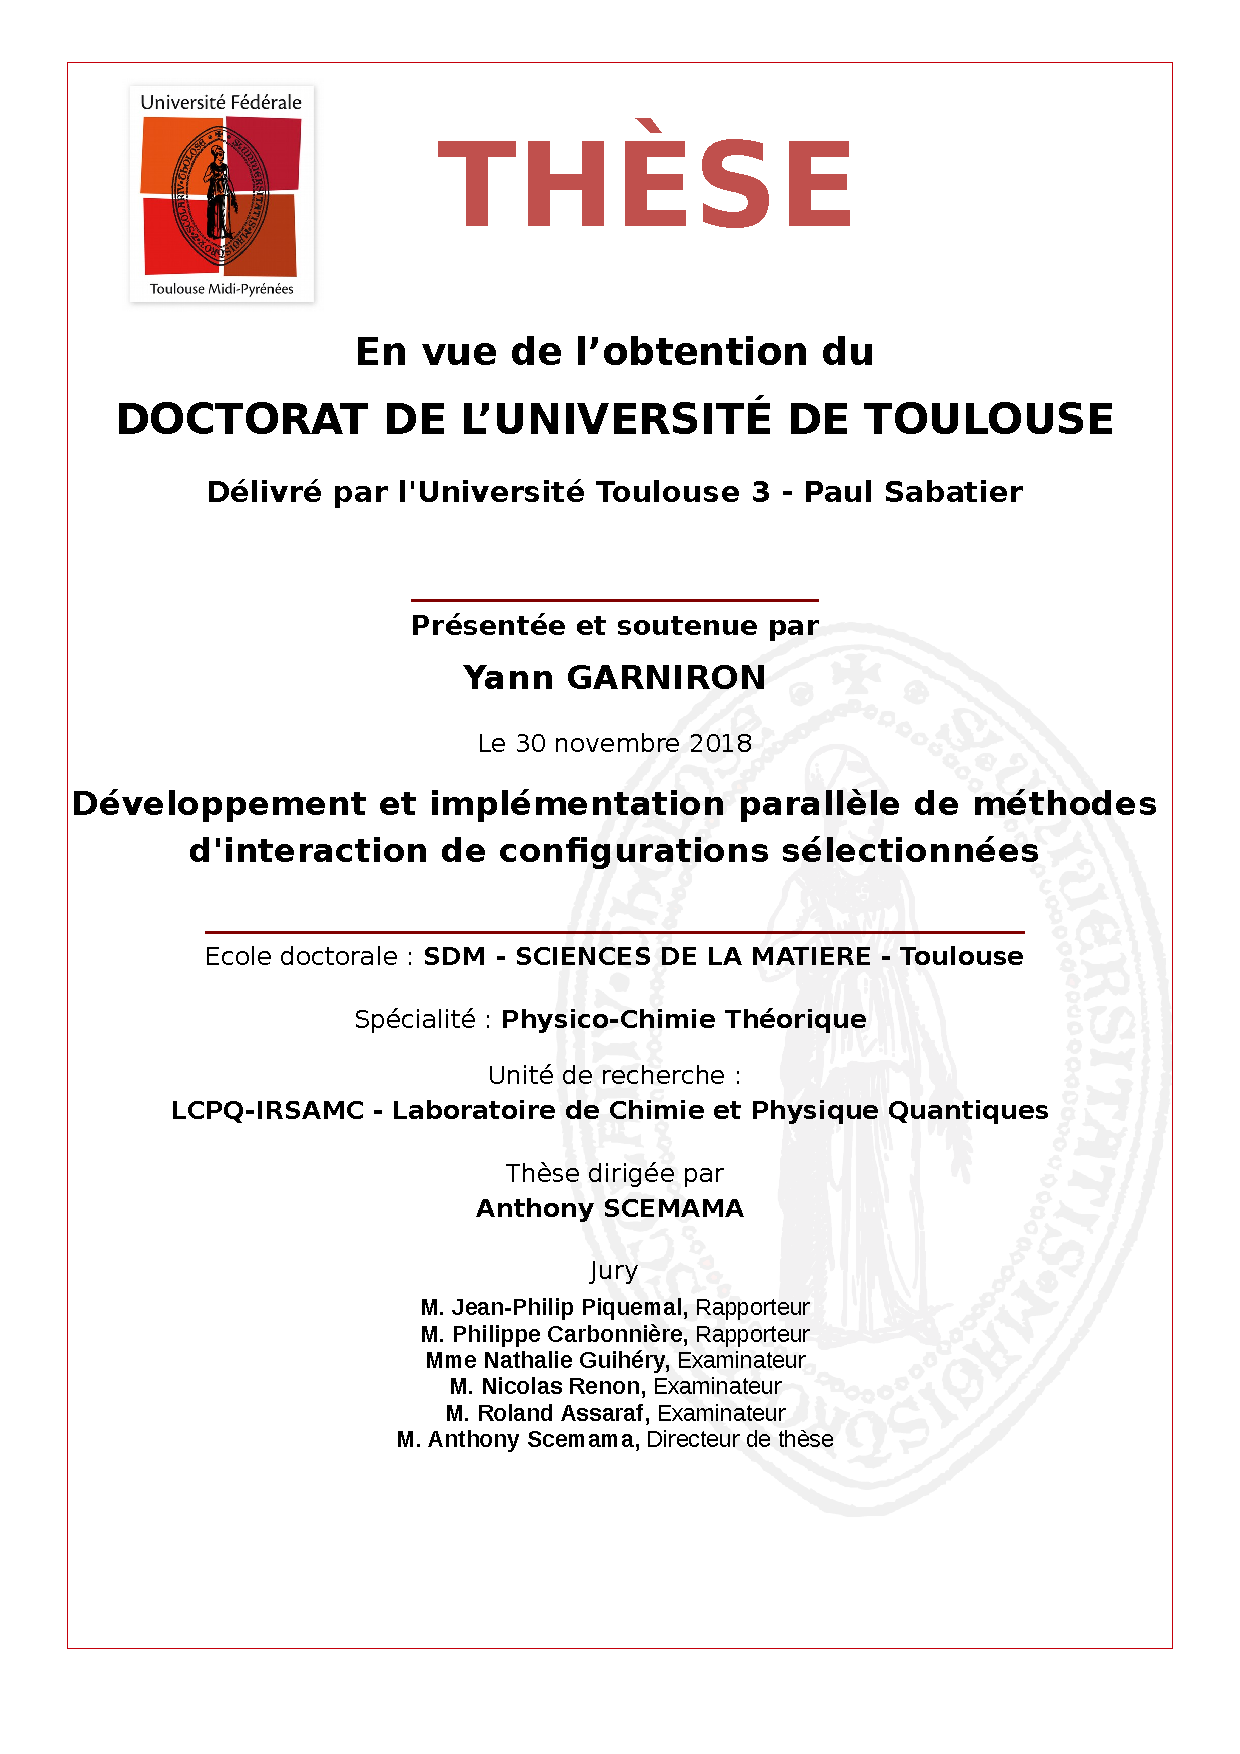
\includepdf{couverture_these}
\newpage

\chapter*{Acknowledgments - PROBLEMS}



%Alors?? Tu n'ecris pas ta these ???


ref au iterative CI voir si c'est la bonne (Nakatsuji ajouté mais pas cité)

citation "Sutter\_2005" dans l'intro ne passe pas...


\newpage

\tableofcontents
\newpage

\section*{Notations}

\begin{itemize}

\item [$\Norb$] Number of molecular orbitals

\item [$\Nst$] Number of considered eigenstates

\item [$\Ndet$] Number of determinants in the internal space

\item [$\Ngen$] Number of generator determinants 

\item [$\Nsel$] Number of selector determinants

\item [$\Nelec$] Number of electrons

\item [$\Nalpha$] Number of $\alpha$-spin electrons

\item [$\Nbeta$] Number of $\beta$-spin electrons

\item [$\Nint$] : Number of 64-bit integers required to store $\Norb$ bits : 
${\Nint = \lfloor \frac{\Norb-1}{64} \rfloor + 1}$

%\item [$\Ndav$] : Number of vectors in the Davidson diagonalization
%
%\item [$\Nperm$] : Number of permutations

\item [$\NFCI$] : Number of determinants in the FCI space

\item [$|\mathcal{D}|$] : Cardinality of the set $\mathcal{D}$.

\item [$\kalpha$] : external determinant
\end{itemize}


%centering in tables



\chapter{Introduction}

During the 3 years I spent at the LCPQ, I worked on improving the Quantum Package, a suit of quantum chemistry code intended for developpers, which focuses on ease of implementation and parallelism.

Quantum chemistry is a field that relies on increasingly expensive computations. The algorithms and approaches proposed in this thesis have been designed in the context of the change in paradigm that has been going on for the last decade,\cite{Sutter_2005} in which the usual sequential algorithms are progressively replaced by parallel equivalents. Indeed, the increase in processors' frequency being challenged by physical barriers, increase in computational power has to be achieved through increase in the number of cores. However, where an increase in frequency mechanically lead to a faster execution of a code, an increase in number of cores may be challenged by algorithmic barriers, which may require adapting of even changing the algorithms.

Initially, this work may been have expected to focus on methods that are by design adapted to massively parallel architectures, such as Monte-Carlo methods (stochastic methods), which are by design composed of a large number of independant tasks (``embarassingly parallel'' algorithms). In addition, they often are able to yield an approximate result for just a fraction of the cost of the equivalent deterministic, exact computation. An example of the move toward this type of method is the recently developped FCIQMC, which can be seen as a Monte-Carlo version of older selection algorithms such as CIPSI, that are iterative and thus a priori not well adapted to parallel architectures. This is however not how things turned out for me.

Many methods, unlike Monte-Carlo ones, are not intrinsically parallel. Nevertheless, some are well-known and widely used, or simply need to be experimented ; and thus they still need to be adapted to parallel architectures. The \QP developped at the LCPQ is a suit of wavefunction quantum chemistry methods, that strives to allow easy implementation and expermientation of new methods, and to make parallel computation as simple as possible. I focused on its improvement all through my thesis, which turned out to be about software developpement at least as much as about quantum chemistry.

The previously mentioned goals of the \QP, in my opinion, have two main consequences
\begin{itemize}
\item
it should be dominantly determinant-driven.
\item
it needs to have some parallel code base for common, deterministic methods.
\end{itemize}


A determinant-driven approach essentially means a wavefunction algorithm loops over determinants rather than electronic integrals, which is usually less effective - due to the larger number of determinants - but also simpler and more intuitive. While the determinant-driven character of the \QP was already established, some improvement was brought to it, in particular for computation of phase factors which, as simple as the problem may seem, is notably time-consuming.

Somewhat logically, the first focus was acceleration and parallelisation of the Davidson diagonalization, which is a pivotal point for CI methods.

The second focus was improvement of the selection algorithm which was the main method used by the \QP to build compact wavefunctions suitable for determinant-driven computations. In a nutshell, the principle is to incrementally build a variational wavefunction by scavenging its external space for determinants that interact with it. While I consider the significant improvement that was brought to this implementation to be in itself the most important part of this work, it also turned out to be the basis for subsequent implementations of other algorithms. Indeed, efficiently implementing this method raised the fundamental question of connecting a variational wavefunction to its external space ; that is, gathering data to go beyond what is readily available in it. The next steps were partly guided by the aversion to waste data gathered during the selection.

Our selection algorithm, CIPSI, implies computing a perturbative contribution for external determinants, and include the ones of largest contribution into the internal (variational) wavefunction. $\EPT$ the sum of all contributions approximates how much energy the variational wavefunction is missing compared to Full-CI energy, which is the exact solution in a given basis set. However to perform an acceptably accurate selection, not all external determinants need to be considered, nor do each contribution needs be known with great accuracy. This allows for approximations too severe for the sum of all computed contributions to yield an accurate estimation $\EPT$. Incidently, computation of $\EPT$ is much more costly that selection. We designed a hybrid deterministic-stochastic scheme which enabled us to get an acceptably accurate value for $\EPT$ by computing a few percent of all contributions.

Computation of $\EPT$ allows to correct the energy of our internal wavefunction by taking into accout its external space. Unfortunately, it only refines the energy and not the wavefunction itself. Based on the shifted-Bk algorithm, and using our CIPSI implementation and the hybrid deterministic-stochastic scheme we designed for computation of $\EPT$, we were able to refine our wavefunction under the effect of a stochastically estimated external space (stochastic matrix dressing).

In addition, we set up a more general framework to enable refining of the variational wavefunction under the effect of a ``custom'', stochastically estimated external space. This was experimented by implementing a MR-CCSD external space.


The efficiency for the implemented algorithms has been studied, and the code could give way to numerous applications, in particular to obtain reference energies for complicated molecular systems.

Of course, the technical considerations were not the focus of the different articles that were produced. In particular, no publication was made about our CIPSI implementation. Because my work focused on the actual implementations of the methods at least as much as on the theory behind them, this thesis is an opportunity to discuss the implementations in more details. In order for it to complete the articles as well as possible, I decided to write it in english.



\chapter{Wave function methods}
\minitoc
\subfile{methods}

\chapter{Determinant-driven computation of the matrix elements}
\minitoc
\subfile{det_driven}

\chapter{Diagonalization with Davidson's algorithm}
\minitoc
\subfile{davidson}

\chapter{Selection with the CIPSI criterion}
\minitoc
\subfile{cipsi}

\chapter{Computation of the second-order perturbative correction}
\minitoc
\subfile{pt2}

\chapter{Stochastic Matrix dressing}
\minitoc
\subfile{matrix_dressing}

\chapter{Application of Stochastic Matrix dressing to MRCC}
\minitoc
\subfile{exp_dressing}

\chapter{Performance measurements}
\minitoc
\subfile{perf}

\chapter{Applications}
\minitoc
\subfile{applications}

\chapter{Conclusion}

As a conclusion, significant improvements were brought to the \QP in both sequential and parallel aspect.

The Davidson diagonalization, which is at the center of many methods, suffers from the impossibility to fully store the Hamiltionian, forcing it to be recomputed on the fly at each iteration. While an extremely fast method was already available to detect zero matrix element,\cite{Scemama_2013} the former implementation still had to iterate over the $~\Ndet^2$ matrix elements. Now, determinants are split in disjoint sets, which are often identifiable as entirely disconnected from one another. Thus only a small fraction of the matrix elements need to be explored.
While the parallelization of this method was somewhat challenging, due to the elementary tasks being extremely unbalanced, a distributed implementation was realized with rather satisfying results.

The CIPSI selection algorithm, whose previous implementation was somewhat naive, was enormously improved, allowing for some applications that were not feasible so far\cite{Scemama_2018,1806.05115}. Several different accelerations were used, reducing the cost of finding connections between external and internal determinant (``batch'' approach, filtering), as well as the cost of computing the corresponding matrix element in the Hamiltonian (phasemask, systematic determination of excitaions). Again, in spite of unbalanced elementary tasks, a distributed implementation could be realized.
Because computation of $\EPT$ was done by the same algorithm but did not allow for as much approximation - and thus was more expensive - a hybrid stochastic-deterministic approach was imagined. $\EPT$ being in itself an approximation for the Full-CI energy, an exact value is indeed not required. Our scheme allows to compute $\EPT$ with an error bar smaller than the typical error bar of $E_{\text{var}} + \EPT$ versus the Full-CI energy, for a few percent of the cost of the deterministic computation.

To get the best of the data we were already able to gather, we implemented the shifted-Bk method, which uses the energy contributions computed by $\EPT$ to refine the internal wavefunction. It essentially creates an external space of determinants $\kalpha$ whose coefficients are perturbatively estimated, and allows them to act on internal coefficients. This method requires computation of a dressing matrix, which we could estimate stochastically in the same way we did for $\EPT$ (stochastic matrix dressing).
The challenge in this case was to estimate, instead of a scalar, a vector of size $\Ndet$, which can be up to a few million elements. The storage and network issues could be solved by setting up a system of predefined checkpoints, a modest drawback being the impossibility to get an estimated dressing matrix outside of those checkpoints.

Finally, this stochastic matrix dressing computation was extended to another external space, that of the Multi-Reference Coupled-Cluster we had previously implemented deterministically,\cite{Garniron_2017} which allowed to explore some possibilities of the bitstring-based determinant-driven approach.



%montagne \cite{Loos_2018}
%sbk \cite{Garniron_2018}
%jmm \cite{Giner_2017}
%mrcc \cite{Garniron_2017}
%pt2 \cite{Garniron_2017b}
%fes \cite{Scemama_2018}
%Cu \cite{1806.05115}

\appendix

\chapter{A Jeziorski-Monkhorst fully uncontracted multi-reference perturbative treatment. I. Principles, second-order versions, and tests on ground state potential energy curves \cite{Giner_2017}}
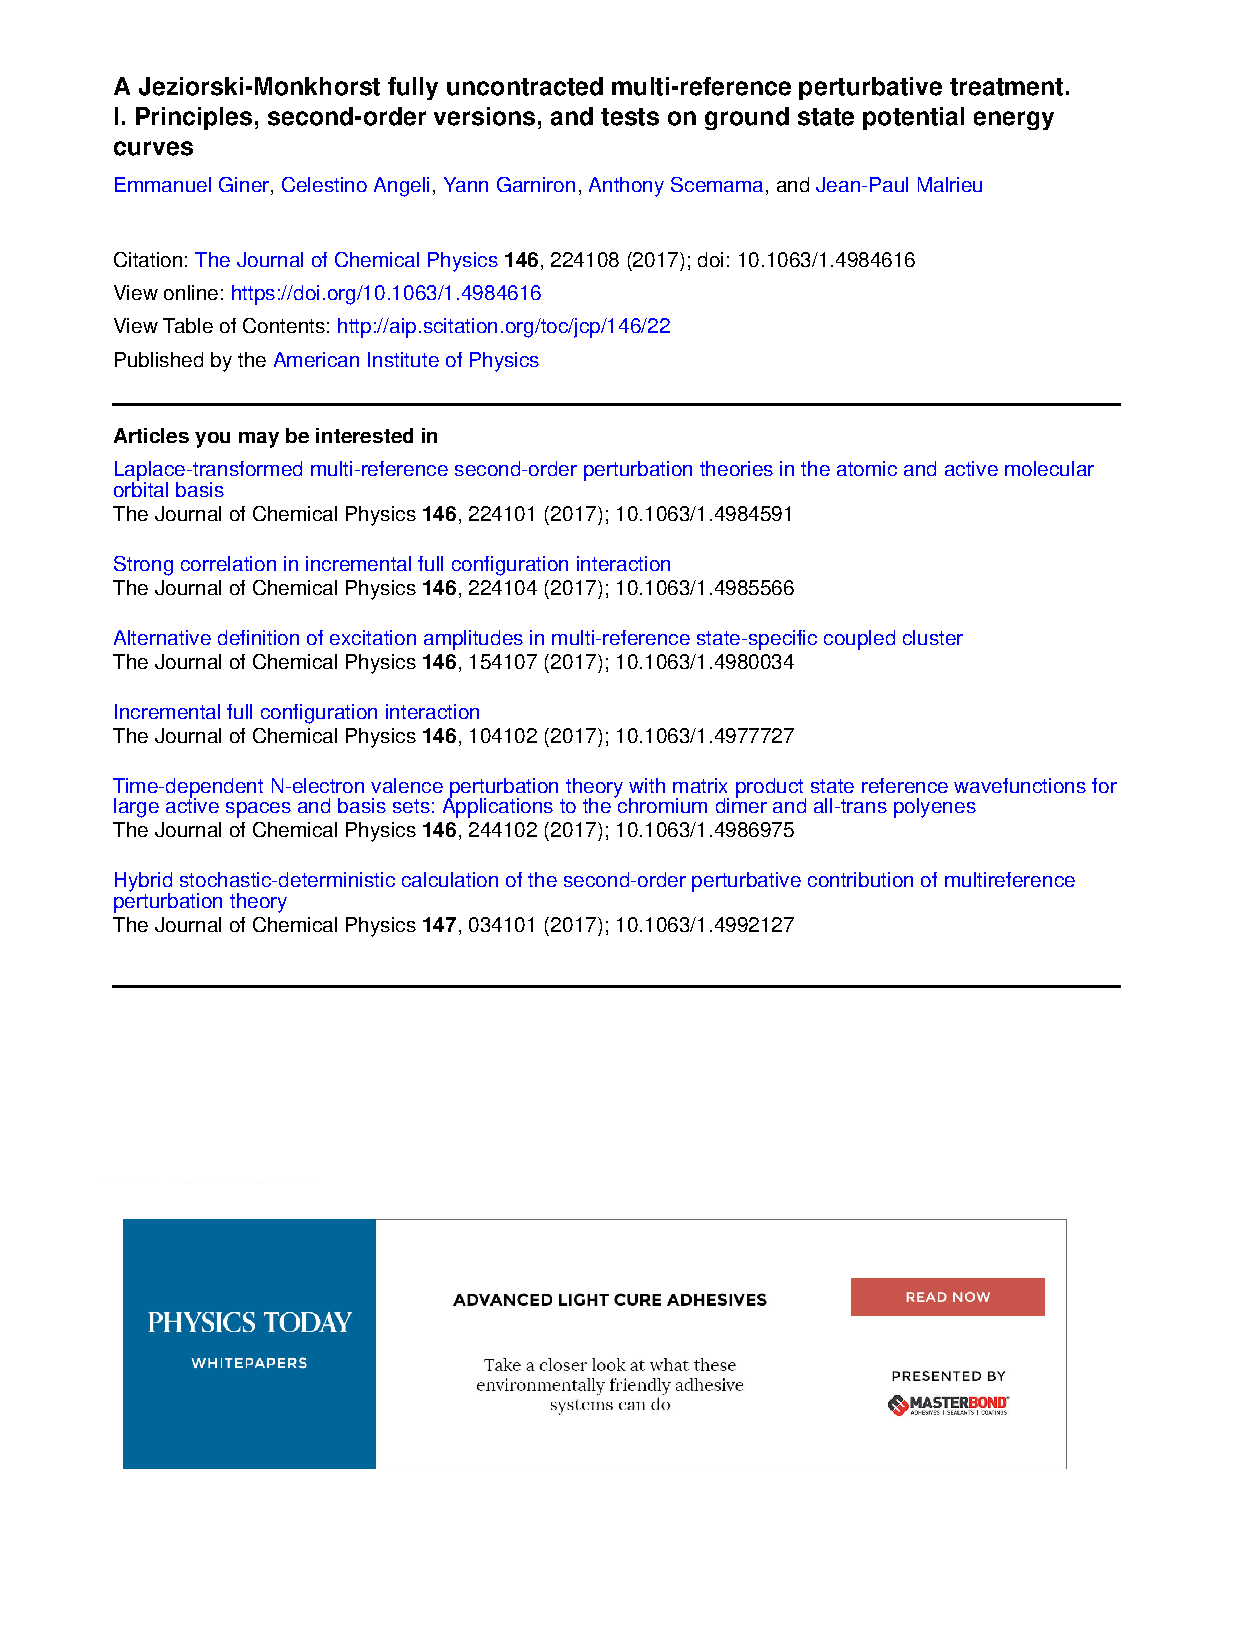
\includepdf[page=2-]{article_jmmrpt2}

\bibliographystyle{ieeetr}
\bibliography{thesis}

%\appendix 
%\chapter{Quantum Package basics}
%\minitoc
%\subfile{qp_general}

\end{document}




